\documentclass[11pt]{article}
\usepackage[utf8]{inputenc}
\usepackage{hanging}
\usepackage{blindtext}
\usepackage{enumitem}
\usepackage{xcolor}
\usepackage{titlesec}

\usepackage
[       a4paper,
        left=3cm,
        right=3cm
] {geometry}



% =====INTERNET CODE COPIED========================

\titleclass{\subsubsubsection}{straight}[\subsection]

\newcounter{subsubsubsection}[subsubsection]
\renewcommand\thesubsubsubsection{\thesubsubsection.\arabic{subsubsubsection}}
\renewcommand\theparagraph{\thesubsubsubsection.\arabic{paragraph}} % optional; useful if paragraphs are to be numbered

\titleformat{\subsubsubsection}
  {\normalfont\normalsize\bfseries}{\thesubsubsubsection}{1em}{}
\titlespacing*{\subsubsubsection}
{0pt}{3.25ex plus 1ex minus .2ex}{1.5ex plus .2ex}

\makeatletter
\renewcommand\paragraph{\@startsection{paragraph}{5}{\z@}%
  {3.25ex \@plus1ex \@minus.2ex}%
  {-1em}%
  {\normalfont\normalsize\bfseries}}
\renewcommand\subparagraph{\@startsection{subparagraph}{6}{\parindent}%
  {3.25ex \@plus1ex \@minus .2ex}%
  {-1em}%
  {\normalfont\normalsize\bfseries}}
\def\toclevel@subsubsubsection{4}
\def\toclevel@paragraph{5}
\def\toclevel@paragraph{6}
\def\l@subsubsubsection{\@dottedtocline{4}{7em}{4em}}
\def\l@paragraph{\@dottedtocline{5}{10em}{5em}}
\def\l@subparagraph{\@dottedtocline{6}{14em}{6em}}
\makeatother

\setcounter{secnumdepth}{4}
\setcounter{tocdepth}{4}




%========== INTERNET COPIED CODE ENDS===============


%\usepackage{indentfirst}
\usepackage{comment}
\usepackage{natbib}
\usepackage{graphicx}
\usepackage{float}
\usepackage{color}   %May be necessary if you want to color links
\usepackage{hyperref}
\setcounter{secnumdepth}{4}
\hypersetup{
    colorlinks,
    citecolor=black,
    filecolor=black,
    linkcolor=black,
    urlcolor=black
}

\renewcommand{\contentsname}{Table of Contents}

\begin{document}


\begin{titlepage}

\newcommand{\HRule}{\rule{\linewidth}{0.5mm}} % Defines a new command for the horizontal lines, change thickness here

%----------------------------------------------------------------------------------------
%	LOGO SECTION
%----------------------------------------------------------------------------------------


%----------------------------------------------------------------------------------------

\center % Center everything on the page

%----------------------------------------------------------------------------------------
%	HEADING SECTIONS
%----------------------------------------------------------------------------------------
\textsc{}\\[3cm] % Name of your university/college
\textsc{\Huge \bfseries Software Design Description}\\[1cm] % Name of your university/college


%----------------------------------------------------------------------------------------
%	TITLE SECTION
%----------------------------------------------------------------------------------------
\makeatletter
\HRule \\[0.4cm]
{ \LARGE  Amazon Go }\\[0.1cm] % Title of your document
\HRule \\[4cm]
 
%----------------------------------------------------------------------------------------
%	AUTHOR SECTION
%----------------------------------------------------------------------------------------

\begin{minipage}{0.4\textwidth}
\begin{flushleft} \large
\emph{Authors}\\
\@author % Your name
\end{flushleft}
\end{minipage}
~
\begin{minipage}{0.4\textwidth}
\begin{flushright} \large
\emph{Student 1:} \\
Alperen ÇAYKUŞ \\[0.5em] % Supervisor's Name
2237170 \\[1.2em] % Supervisor's Name

\emph{Student 2:} \\
Aytaç Anıl Durmaz \\[0.5em] % Supervisor's Name
2237295 \\[1.2em] % Supervisor's Name
\end{flushright}
\end{minipage}\\[2cm]
\makeatother

% If you don't want a supervisor, uncomment the two lines below and remove the section above
%\Large \emph{Author:}\\
%John \textsc{Smith}\\[3cm] % Your name

%----------------------------------------------------------------------------------------
%	DATE SECTION
%----------------------------------------------------------------------------------------

%{\large \today}\\[2cm] % Date, change the \today to a set date if you want to be precise

\vfill % Fill the rest of the page with whitespace

\end{titlepage}


\newpage

\begin{center}
    \Huge{Change History} 
\end{center}{}
 


\begin{table}[H]
\begin{center}
    

\begin{tabular}{|l|l|}
\hline
\textbf{\Huge{Version}} & \textbf{\Huge{Date}}  \\ \hline
 %
\end{tabular}
\end{center}
\end{table}

\newpage



\begin{flushleft}
    \tableofcontents
\end{flushleft}

\newpage

\begin{flushleft}
    \listoffigures
\end{flushleft}

\newpage

\begin{flushleft}
    \listoftables
\end{flushleft}

\newpage


\section{Introduction}

    \subsection{Purpose of the System}

    % Copied from the SRS. Ask if this is valid.
    The purpose of this system, namely 'Amazon Go', is to enable customers to shop without making them wait in line with a few
    requirements only, which are a smart phone and an Amazon account with a registered credit card. To achieve this purpose, Amazon has opened lots of stores, 
    which are highly equipped with cutting edge sensors and cameras. These cameras and sensors track the customer and products,
    and after the customer is done with shopping, she/he just walks out of store. The amount of his/her shopping will be automatically 
    deduced from his/her specified payment method.
        

    \subsection{Scope}
        \begin{itemize}
        \item System will have a mobile application, which will enable users (i.e, store customers) to interact with the system. 
            Customers will log in to store by using the QR code provided to them by their mobile application. 
            Mobile application is also the place where customers sign up to the system, see their current cart status, and past shoppings.
        \item System will use remote servers to keep data of the customers, such as current shopping session, payment information, etc. 
            Remote server will also communicate with the mobile application to enable a customer to see his/her current shopping session, 
            past shoppings, etc. 
        \item System will have physical stores, which are equipped with very sensitive sensors and cameras. Using Artificial Intelligence 
            and Computer Vision algorithms, these cameras and sensors will gather information from the store and communicate with the remote server.
        
        \item System will use several APIs to communicate with the specified payment method of the customers, such as bank accounts. 
            By doing so, system will be able to withdraw money from the customer's account when she/he is done with shopping.
        
        \item System will use a database to store customer related information (such as user ID), temporary customer shopping cart, store workers' information,
            products' information and a database table for the system admins. Those mentioned tables such as customer related information 
            actually consist of multiple tables. Only the system admins are able to make changes and read the database.
        
        \item System will keep log of all the shoppings of the users on the remote server for legal purposes. Only system admins can see these logs.
        
        \item System will also have a store worker interface to enable the store worker to troubleshoot in case something goes wrong in the store, 
        such as sensor malfunctioning, incorrect amount of money withdrawn from the customer, wrong product was added to a customer's cart, etc.
        \end{itemize}



    \subsection{Stakeholders and their concerns}
        \begin{itemize}
            
            \item {\textbf{Amazon:}}
                Being the owner of the whole system and the store, Amazon's main concern is reliability of the system so that Amazon will 
                not lose money due to sensor failures or due to customers tricking the sensors and being charged less than they are supposed to be charged.
                Privacy of the customers is also important as this may have legal consequences.

            \item {\textbf{Users:}}
                Users are actually the customers that visit Amazon GO stores. They have four main concerns, which are, firstly, not waiting 
                in line to pay for what they had bought; secondly, precision of the sensors so that they do not pay extra money
                due to sensors' fault; thirdly, security of their personal information such as their credit card information, place of residence etc., 
                which are stored in the Amazon servers; and lastly, having a mobile application which is easy to use.
               
            \item {\textbf{System Developers:}}
                Developers are very critical for this system, because it completely relies on the software. Their main concern is maintainability, due
                to complexity of the system. For this purpose, the documentation and the system itself should be organized very well. Also, the system 
                must be set up in a way that if one component fails, restoration of this component and integration of the new component, which replaces the 
                faulty one, with the system must be easy.

            \item {\textbf{IT Staff:}}
                IT Staff are basically the system administrators, who are responsible to maintain databases and communicate with the store workers when needed.
                They are essential in the continuity of the system. Their major concern is that sustainability of the database, which is created by the system
                developers when the system is being developed. 

            \item {\textbf{Store Workers:}}
                Store workers are the people that are responsible for the product placement and shelf maintenance. They are mostly concerned about the 
                illegal actions. Therefore, they should be trained to what to do for the most of the possible scenarios. 
                Their main concerns are being able to easily reach a system admin in case of a failure, and being able to contact with the security
                in case of an illegal action by the customers.  
        \end{itemize}

\section{References}
%% @@@@@@@@@@@@@@@@@@@@@@@@@@@@@@@@@@@@ OLD REFERENCES !!!!!
\textbf{This document is written with respect to the specifications of the document below:\\}

1016-2009 - IEEE Standard for Information Technology--Systems Design--Software Design Descriptions
$$ $$ 
\setlength{\parindent}{1 cm}
\textbf{Other sources:\\}
\begin{hangparas}{1cm}{1}
 \par
 Cheng, A. (2019, January 13). Why Amazon Go May Soon Change The Way We Shop. Retrieved from \textit{https://www.forbes.com/sites/andriacheng/2019/01/13/why-amazon-go-may-soon-change-the-way-we-want-to-shop} 


 \par
 Wingfield, N. (2018, January 21). Inside Amazon Go, a Store of the Future.\\ 
 Retrieved from \textit{https://www.nytimes.com/2018/01/21/technology/inside-amazon-go-a-store-of-the-future.html }
   
\end{hangparas}

\section{Glossary}
\begin{table}[H]
    \begin{center}
    \begin{tabular}{|p{5cm}|p{8cm}|}
    \hline
    \textbf{Term} & \textbf{Definition}   \\ \hline
    User & A customer that is signed up to Amazon Go application and has a unique user ID. \\ \hline
    
    Database & A MySQL database.  \\ \hline
    User ID & A unique number which can be used to identify a user.  \\ \hline
    Store Worker & A real person working in an Amazon Go store.  \\ \hline
    API & Application Programming Interface   \\ \hline
    %HTTPS & Hypertext Transfer Protocol Secure  \\ \hline
    %TCP & Transmission Control Protocol \\ \hline
    Mobile Application & An application that must be installed to an Android or iOS device in order to access Amazon GO features.\\ \hline
    QR Code & An image which contains information about the user. It is generated by the mobile application.  \\ \hline
    System admins  & The people who are responsible for the maintenance and the order of the Amazon GO system.   \\ \hline
    Remote server & A real physical computer away from the stores, at the Amazon HQ, which can be accessed via SSH by system admins.   \\ \hline
    SSH & Secure Shell   \\ \hline
    Sensor & A physical electronic device that collects information about the environment it is currently in.   \\ \hline
    Product & The goods that are sold at the Amazon GO stores.   \\ \hline
    % &   \\ \hline

    \end{tabular}
    \caption{Glossary}
    \label{glossary}
      \end{center}
\end{table}

\newpage

\section{Architectural Views}
    \subsection{Context View}

    In this viewpoint, the systems that Amazon GO interacts with are shown on the \nameref{contextDiagram} below. The following \nameref{ucaseDiagram} 
    shows the actors and their possible interactions with different scenarios. The detailed information about these use case functions can be found
    on the tables after the Use Case Diagram. These tables give detailed information for each use case function including alternative scenarios.
    During the implementation, these tables shall be considered and implementation must follow the mentioned scenarios.

    \begin{center}
        \begin{figure}[H]
            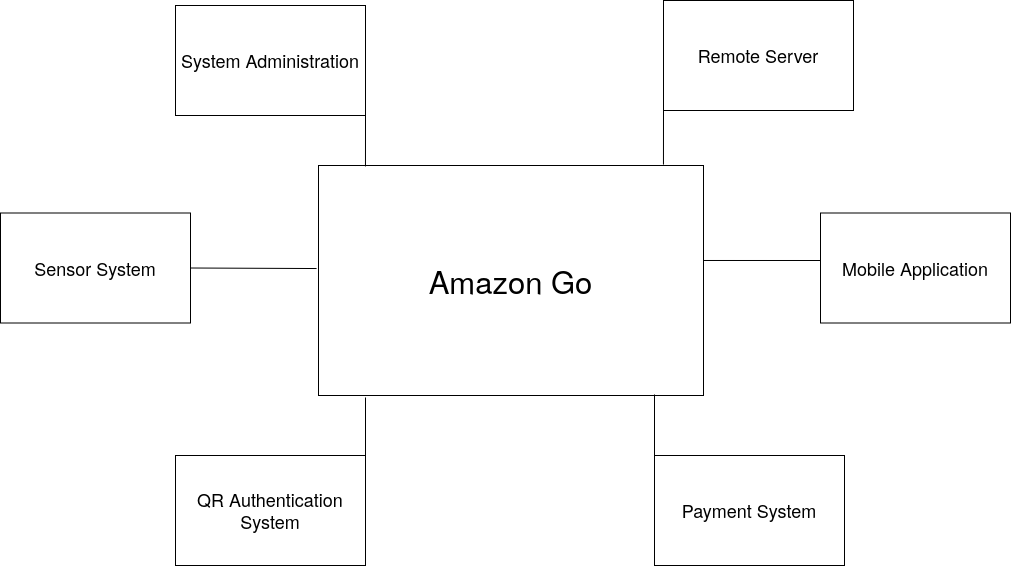
\includegraphics[width=\linewidth]{Images/contextDiagram.png}
            \caption{Context Diagram}
            \label{contextDiagram}
        \end{figure}
        \end{center}

    \begin{center}
        \begin{figure}[H]
            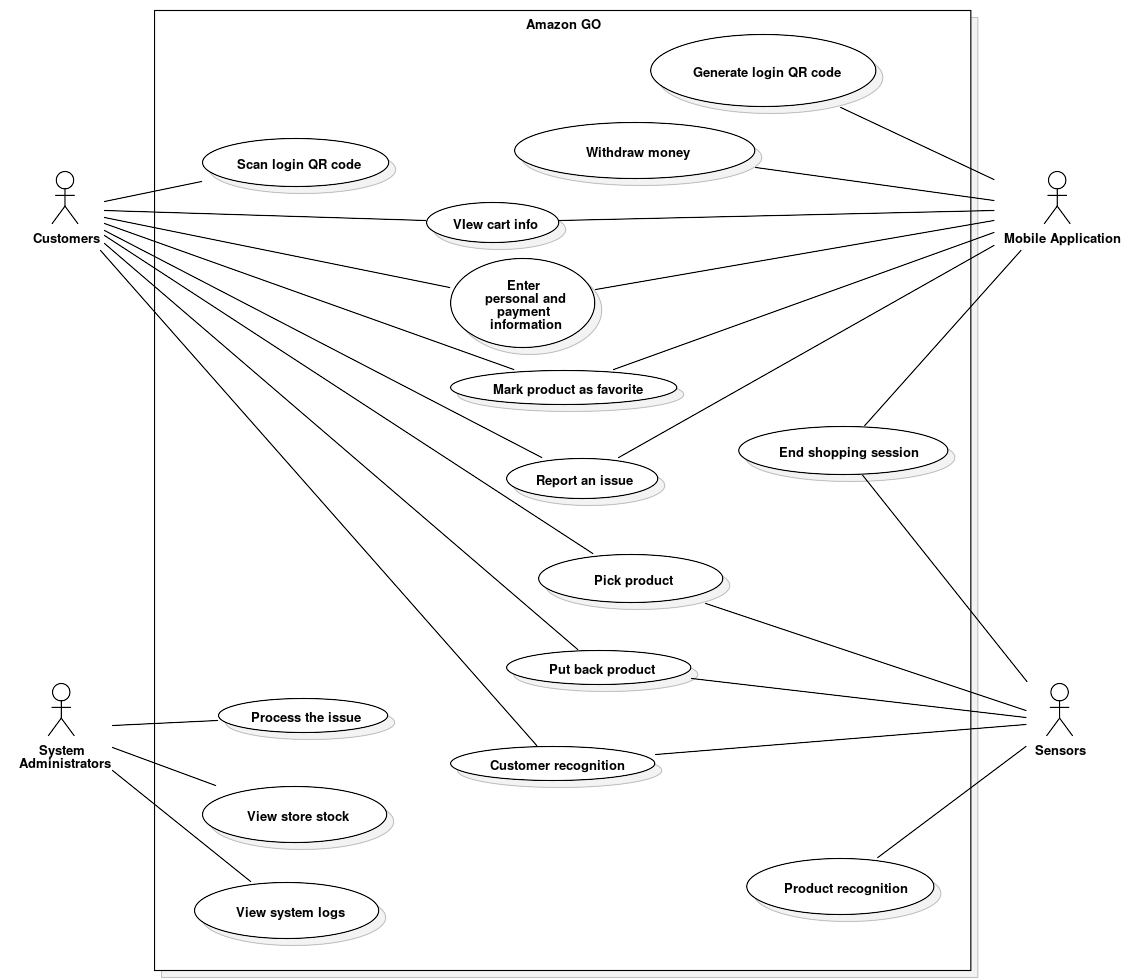
\includegraphics[width=\linewidth]{Images/UseCaseDiagram.png}
            \caption{Use Case Diagram}
            \label{ucaseDiagram}
        \end{figure}
        \end{center}



    \subsection{Composition View}
    \subsection{Information View}
    \subsection{Interface View}






\end{document}




% ========== MIGHT BE NECESSARY==================%

%``I always thought something was fundamentally wrong with the universe'' \citep{adams1995hitchhiker}
%\bibliographystyle{plain}
%\bibliography{references}
